\renewcommand{\thechapter}{\roman{chapter}}
\setcounter{chapter}{4}
\setcounter{figure}{0}

\unchapter{Préambule multimodalité}
\label{chap:preamble_multimodal}
Lors de la partie précédente partie consacré à la microscopie confocale, \Cref{part:microscopy}, différentes méthodes sont proposées afin d'obtenir des prédictions au niveau des images mais surtout des lésions. Cette troisième et dernière partie va nous permettre de mettre au point et d'évaluer des stratégies permettant la mise en place de processus multimodaux d'aide au diagnostic des lésion malignes, mais surtout des lésions de type \gls{lm} et \gls{lmm}. A cette fin, ce préambule présente lors des prochains paragraphes les données employées à cet effet et reprend les points important de l'étude clinique de référence.\par

Pour rappel, les données de photographie clinique et de dermatoscopie ont été mises de côté lors des expériences sur la \gls{rcm} menée lors de la \Cref{part:microscopy}. Ainsi, cette nouvelle partie intègre l'ensemble des données de lésions obtenues dans le cadre de l'étude de Cinotti et al.~\cite{Cinotti2018}, soit 223 lésions pour lesquelles sont mises à disposition les acquisitions issues des modalités de \textit{photographie clinique}, de \textit{dermatoscopie} et \acrlong{rcm}. Ces données sont focalisées autour de lésions malignes de type \gls{lm} et de \gls{lmm} mais également de lésions bénignes proches de celles-ci suceptibles d'induire le praticien en erreur.\par 

De manière plus détaillée, chaque lésion issue de ce jeu de données comporte~:
\begin{itemize}
    \item des données de \textbf{photographie clinique}, \textit{une image par lésion}. Pour 5 de ces lésions, plusieurs images de photographie clinique étaient fournies, seule la plus pertinente d'entre elle a été conservée. De plus, aucun protocole ne régit leur acquisition ce qui abouti à une grande diversité d'images, dont la lésion ne représente parfois qu'une faible portion de l'acquisition. Ainsi, ces images sont recadrées manuellement pour l'objet de ce travail, afin de limiter cette diversité. La résolution spatiale de ces images recadrées est comprise entre 250 $\times$ 250 pixels pour les plus petites d'entre elles à plus de 2000 $\times$ 2000 pixels pour les plus conséquentes.
    \item des données de \textbf{dermatoscopie}, \textit{une image par lésion}. Ces images sont utilisées de manière brute, aucun traitement de ces images n'a été jugée nécessaire. 1920*1080
    \item des données de \textbf{\gls{rcm}}, dont le nombre varie \textit{de quelques images à plusieurs centaines par lésion}. Pour chaque lésion, ces images sont sélectionnées par deux des trois médecins investigateurs de l'étude~\cite{Cinotti2018}. Ces données proviennent essentiellement de la \gls{dej}, particulièrement adapté à l'observation de ce phénomène.
\end{itemize}

% Du point de vue de leurs caractéristiques, ces images arborent une taille constante de 1000 px×1000 px pour une section mesurée de 920μm×920μm pour une résolution en profondeur com-prise entre 3μm–5μm. Ces données fournissent ainsi une résolution de l’ordre du 1μm. Les infor-mations d’acquisition (profondeur, longueur d’onde, . . . )  contenues dans les images ne pourrontêtre utilisées car non exploitables (procédure de calibration non réalisée, informations manquantes,. . . ).

\begin{figure}[H]
    \begin{center}
        \includegraphics[width=\linewidth]{contents/iii_preamble_multimodal/resources/example_clinical_crop.pdf}
        \caption{Exemples de données de photographie clinique recadrées manuellement pour le besoin de cette étude.}
        \label{fig:example_clinical_crop}
    \end{center} 
\end{figure}\par

\begin{figure}[H]
    \begin{center}
        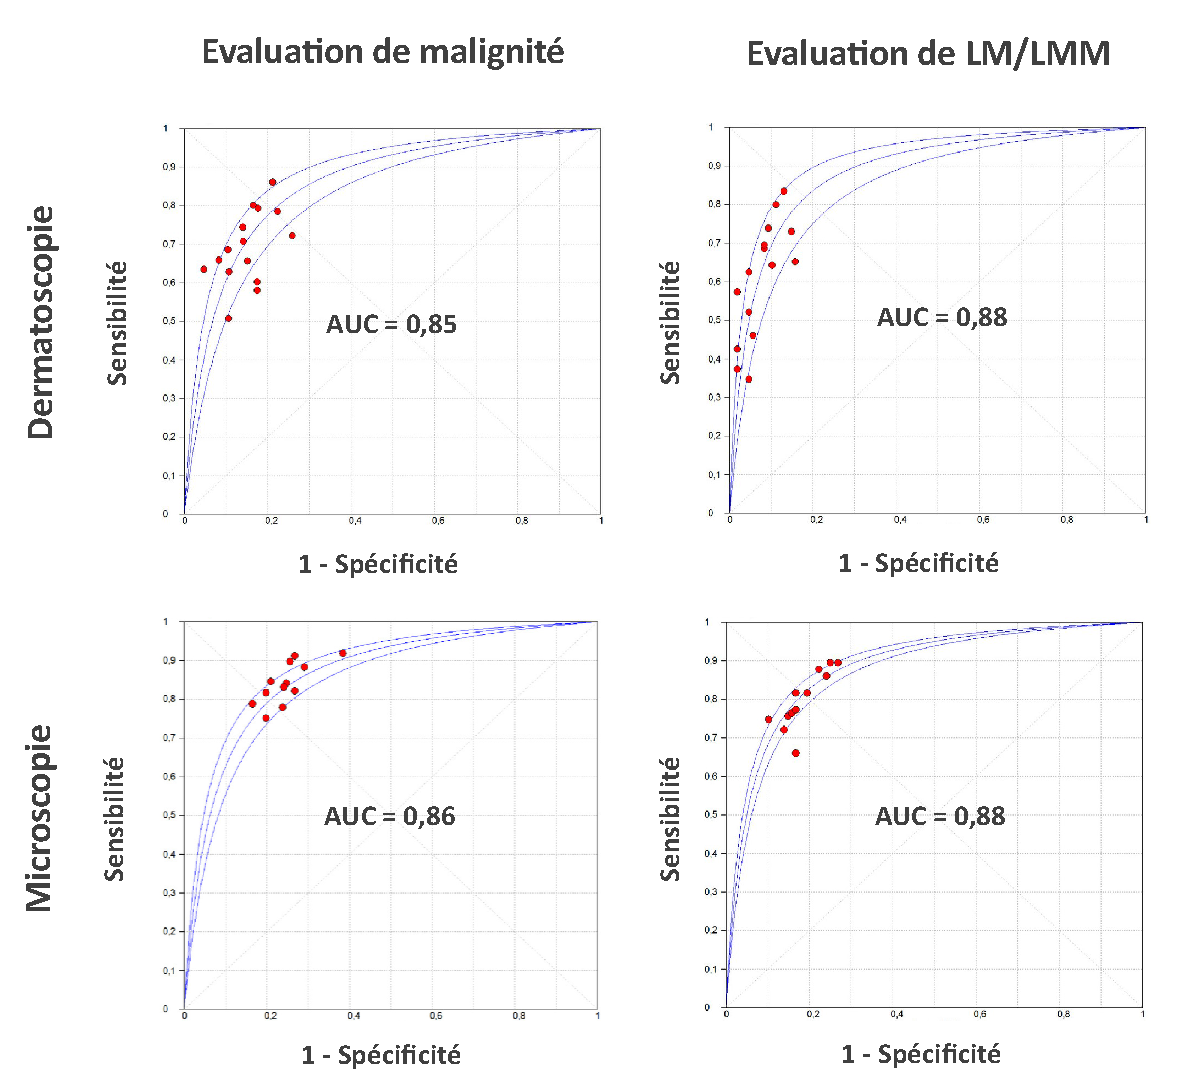
\includegraphics[width=\linewidth]{contents/iii_preamble_multimodal/resources/results_roc_experts.pdf}
        \caption{Résultats .}
        \label{fig:results_roc_experts}
    \end{center} 
\end{figure}\par
 
L'objectif visé par cette partie sera d'égaler ces scores à l'aide de nos méthodes de diagnostic sur base d'images issues de \gls{rcm}. A ce titre, nous n'exploiterons pas les méta-données issues des informations patient bien que utilisées par les spécialistes lors de l'évaluation. Ainsi, l'âge, le sexe ou encore l'emplacement sont autant de critères que nous ne considérerons pas au sein de ces prochains paragraphes bien que employés par les dermatologues experts en \gls{rcm} durant leur évaluation. De plus, contrairement aux connaissances des experts, ces méta-données ne sont pas représentatives de la population réelle, et biaiseraient nos méthodes par des corrélations non valides dans le monde réel dû à l'acquisition de la base de données.\par

% Images were acquired by 3 experts of non invasive skin imaging (JLP, BL or EC). Dermoscopy was performed with the PowerShot® G7 camera (Canon Powershot®, Canon, New York, USA) combined with the FotoFinder Systems (FotoFinder Systems GmbH, Bad Birnbach, Germany). In vivo RCM examination was carried out with the hand-held VivaScope 3000® camera (Caliber Imaging and Diagnostics, New York, USA, distributed in Europe by MAVIG GmbH, Munich, Germany) which uses a laser with a wavelength of 830 nm and images up to 250 µm of depth. Each RCM image corresponds to a horizontal 920 µm x 920 µm section of the skin at a selected depth with a lateral resolution of 1 μm and axial resolution of 3–5 μm. Only images considered relevant for the diagnosis by two out of the three investigators were captured by RCM. Images of different depths (epidermis, dermal-epidermal junction and dermis) were always present.

Afin de répondre à ces objectifs et de clore l'objet de ce manuscrit, cette partie dédiée à la multimodalité propose diverses approches en cascades suceptibles de convenir à des applications en milieu clinique. Ainsi, ces éléments sont étudiées au sein du \Cref{chap:chapter_8} dont il propose une \textbf{prise de décision au niveau lésionnel par uttilisation de processus multimodal}.\par